\documentclass[11pt]{beamer}
\usetheme{Singapore}
\usepackage[utf8]{inputenc}
\usepackage[french]{babel}
\usepackage[T1]{fontenc}
\usepackage{amsmath}
\usepackage{amsfonts}
\usepackage{amssymb}
\usepackage{minted}
\usepackage{changepage}

\author{Le groupe MkRpg}
\title{Présentation du projet MkRpg}
%\setbeamercovered{transparent} 
\setbeamertemplate{navigation symbols}{} 
\renewcommand{\insertnavigation}[1]{\hfill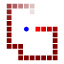
\includegraphics[scale=.5]{main.png}~\vspace{-.3cm}}
% Raoul :
%\renewcommand{\insertnavigation}[1]{\hfill
\includegraphics[scale=.25]{raoul.png}~\vspace{-.2cm}}
%\setbeamertemplate{headline}{}
%\logo{} 
%\institute{} 
%\date{} 
%\subject{} 
\begin{document}

\begin{frame}
\titlepage
\end{frame}

\begin{frame}{Sommaire}
\tableofcontents
\end{frame}

%%%%%%%%%%%%%%%%%%%%%%%%%%%%%%%%%%%%%%%%%%%%%%%%%%%%%%%%%%%%%%%%%%%%%%


\section*{Introduction}

\begin{frame}
    \frametitle{\secname}
    \begin{itemize}
        \item A game is described by XML files
        \item Need to parse and get the whole data in a quite safe way
        \item Create all instances of a game with  the parsed data.
    \end{itemize}
\end{frame}

\begin{frame}
    \frametitle{\secname~: What is needed.}
    \begin{itemize}
        \item Define a format for the XML files that is compliant with the
            expectations.
        \item Have it general enough for description, and usable in order to
            generate the instances.
        \item Use the good data structures in order to keep parsed data.
        \item Generate instances.
    \end{itemize}
\end{frame}

\section{Parsing XML files}
\subsection{XML description files}

\begin{frame}
    \frametitle{What needs to be defined}
    \begin{itemize}
        \item Interactions~:reaction to the keys
        \item Actions~: Link between interactions and the world, reaction to
            collision,\dots
        \item Objects~: Entities, objects, maps, cells,\dots
    \end{itemize}
\end{frame}


\subsubsection{Actions}

\begin{frame}[fragile]
    \frametitle{\subsecname}
    \begin{figure}
        \begin{adjustwidth}{0.1\textwidth}{}
            \scriptsize{\inputminted{xml}{test_files/actions.xml}}
        \end{adjustwidth}
        \caption{An Action XML tag}
    \end{figure}
    \begin{small}
        \begin{adjustwidth}{-0.1\textwidth}{}
            \begin{description}
                \item[Event] is the interaction that triggers this action.
                \item[Order] is the orders to be executed~:
                    \begin{description}
                        \item[Target] is the target of the action
                        \item[Param] is the parameter to be modified by the
                            action.
                        \item[Value] is the code to be runned. (Yes, by
                            \verb|eval|)
                    \end{description}
            \end{description}
        \end{adjustwidth}
    \end{small}
\end{frame}

\subsubsection{Interactions}

\begin{frame}
    \frametitle{\subsecname}
    \begin{figure}
        \begin{adjustwidth}{0.1\textwidth}{}
            \scriptsize{\inputminted{xml}{test_files/interactions.xml}}
        \end{adjustwidth}
        \caption{An Interaction XML tag}
    \end{figure}
    \begin{small}
        \begin{description}
            \item[Key] is the \emph{keycode} associated to the interaction
            \item[Target] is the target of the interaction~: the player, the
                map,\dots
            \item[Event] is the event to be triggered by the action
        \end{description}
    \end{small}
\end{frame}

\subsubsection{Entities}

\begin{frame}
    \frametitle{\subsecname}
    \begin{figure}
        \begin{adjustwidth}{0.1\textwidth}{}
            \scriptsize{\inputminted{xml}{test_files/entity.xml}}
        \end{adjustwidth}
        %\caption{An Entity XML tag}
    \end{figure}
    \begin{small}
        \begin{adjustwidth}{-0.1\textwidth}{}
            \begin{description}
                \item[Ident] is the numerical identifier of the entity
                \item[Params] describes the parameters of an entity~:
                    \begin{description}
                        \item[Picture] an identifier corresponding to the image
                            representing the character.
                        \item[X, Y] are the starting coordinates
                        \item[Map] is the map on which the entity should be
                            when starting a game.
                    \end{description}
            \end{description}
        \end{adjustwidth}
    \end{small}
\end{frame}

\subsection{Parsing XML Files}

\subsubsection{Parsing with Python}

\begin{frame}[fragile]
    \frametitle{\subsecname}
    \begin{block}{Library}
        Use the python library \verb|xml|, more precisely
        the module \verb|xml.etree.ElementTree|
    \end{block}
    The parser is integrated, most of the work consisted in organizing
    the parsing, and finding the good data structures.
    A big work also was to keep a general enough parsing.
\end{frame}

\subsubsection{Formatting data}

\begin{frame}[fragile]
    \frametitle{\subsecname}
    \begin{alertblock}{First try}
        Use \verb|dict|. However, dicts iterates in an arbitrary order,
        so the \verb|id|s weren't the same client-side and server-side
    \end{alertblock}

    \pause

    \begin{alertblock}{Second try}
        \verb|dict| and \verb|id|s in the xml. It still fails
        since some data was created at runtime with different \verb|id|s.
    \end{alertblock}

    \pause

    \begin{block}{Third try}
        Use \verb|collection.OrderedDict|s in order to solve
        all the issues.
    \end{block}
\end{frame}


%%%%%%%%%%%%%%%%%%%%%%%%%%%%%%%%%%%%%%%%%%%%%%%%%%%%%%%%%%%%%%%%%%%%%%
\section{Interface}
    \begin{frame}
        \frametitle{Contents}
        \tableofcontents[currentsection]
    \end{frame}

\begin{frame}{Architecture}
	\begin{center}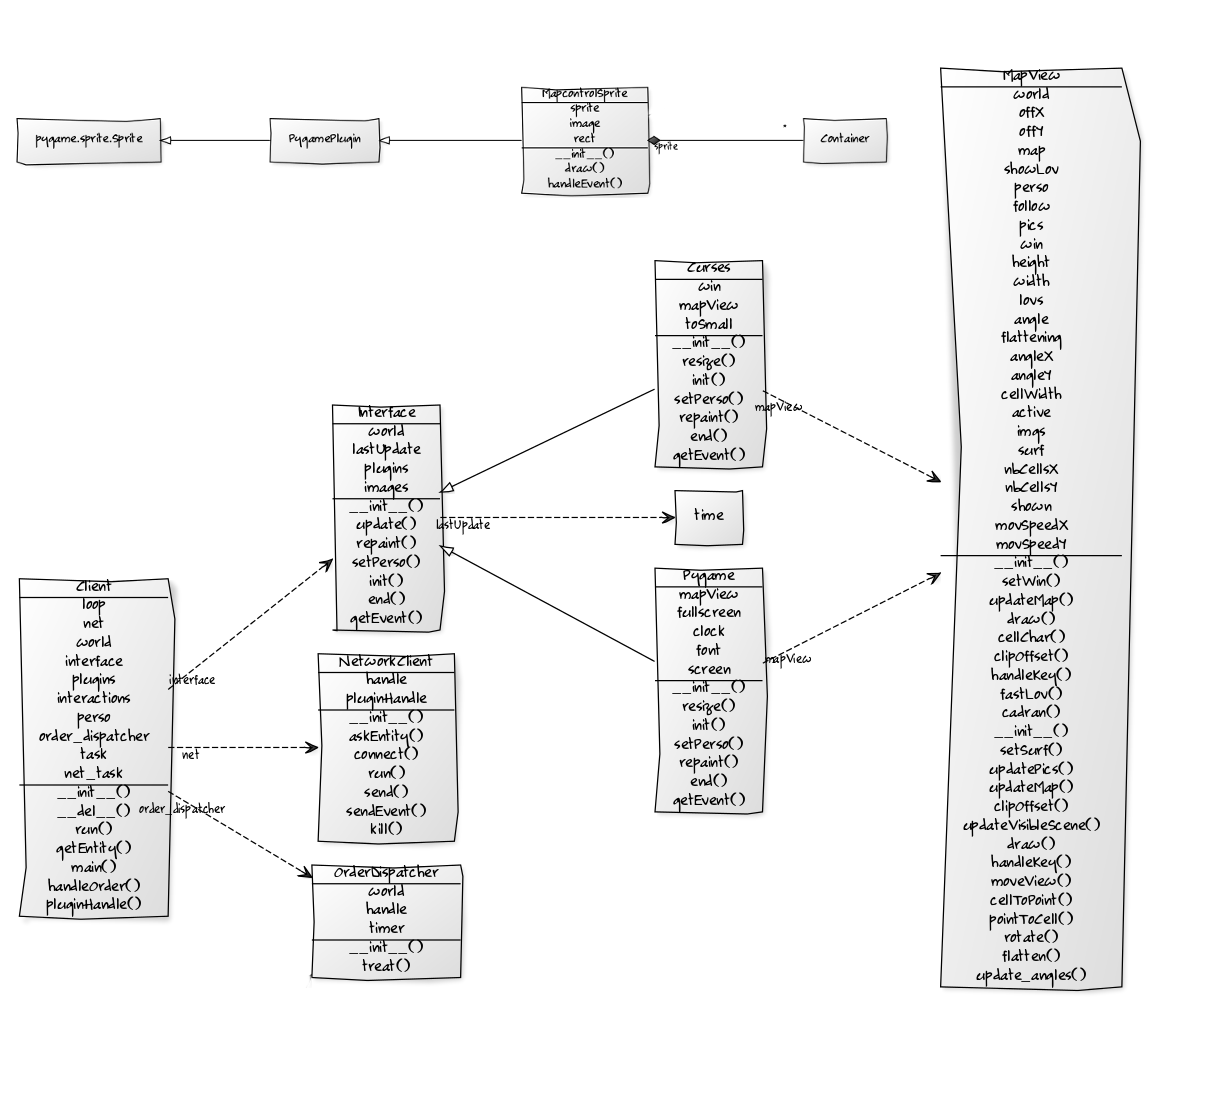
\includegraphics[scale=0.21]{uml_pygame.png}\end{center}
\end{frame}

\begin{frame}{Interface pygame : features}
	\begin{itemize}
		\item mise en cache
    \item changement de cartes
    \item rotation de carte
    \item zoom/dezoom
    \item affichage d'objets
    \item système de gui
    \item plugins d'affichage
	\end{itemize}
\end{frame}

\begin{frame}{Interface pygame}
	\begin{itemize}
    \item performances : raisonnables, 30 FPS, quelques lags quand on affiche des parties trop importantes de la map
		\item[]
    \item stabilité : quelques exceptions non capturées (rotation de carte), sinon affichage très stable
	\end{itemize}
\end{frame}

\begin{frame}{Interface pygame}
	\begin{center}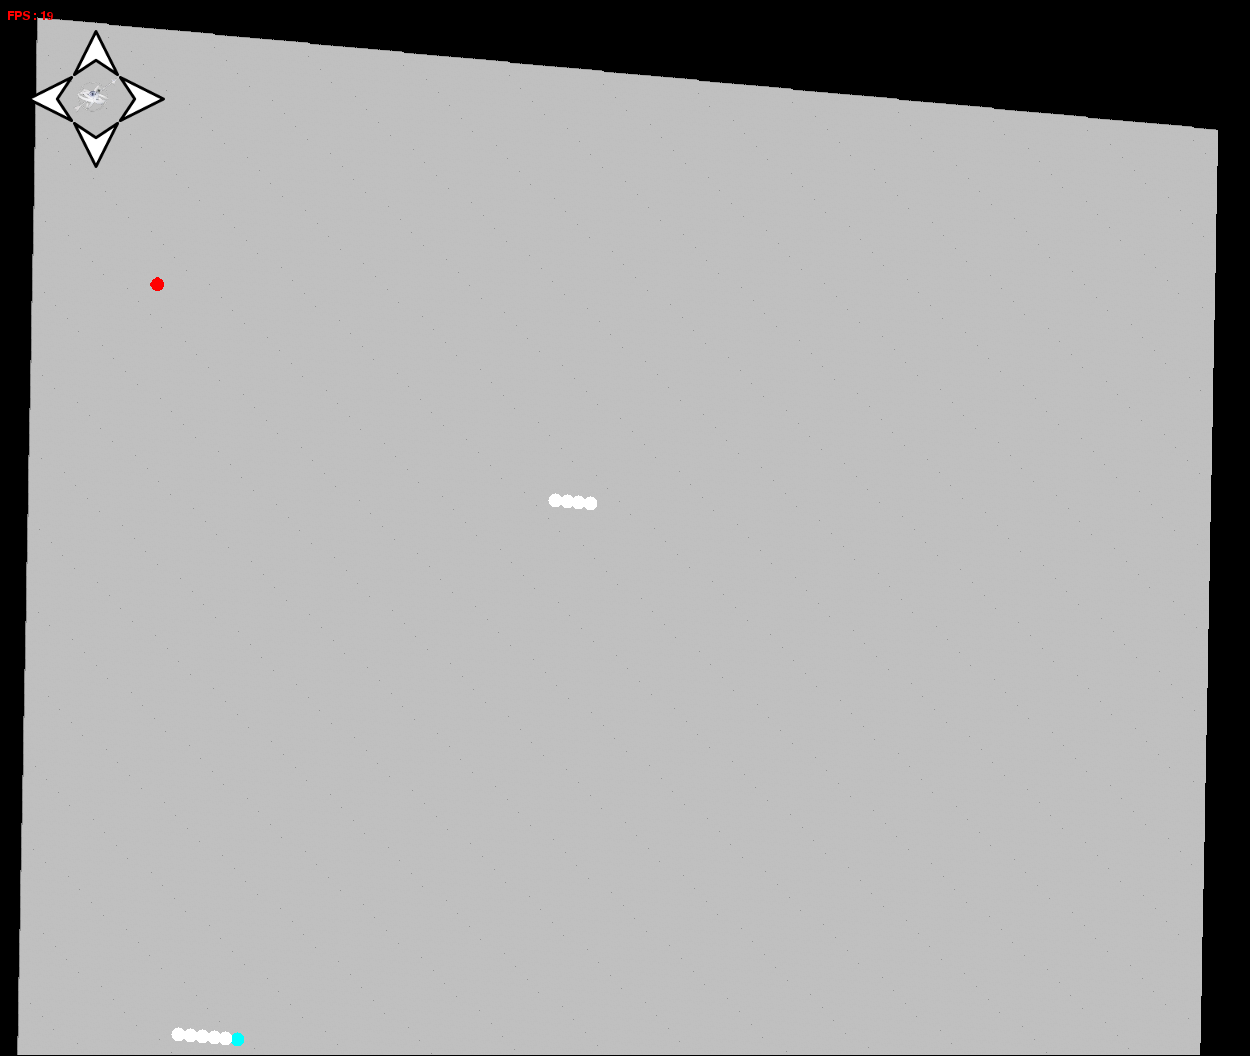
\includegraphics[scale=0.2]{game_screenshot.png}\end{center}
\end{frame}

\begin{frame}{Interface pygame : GUI}
	\begin{center}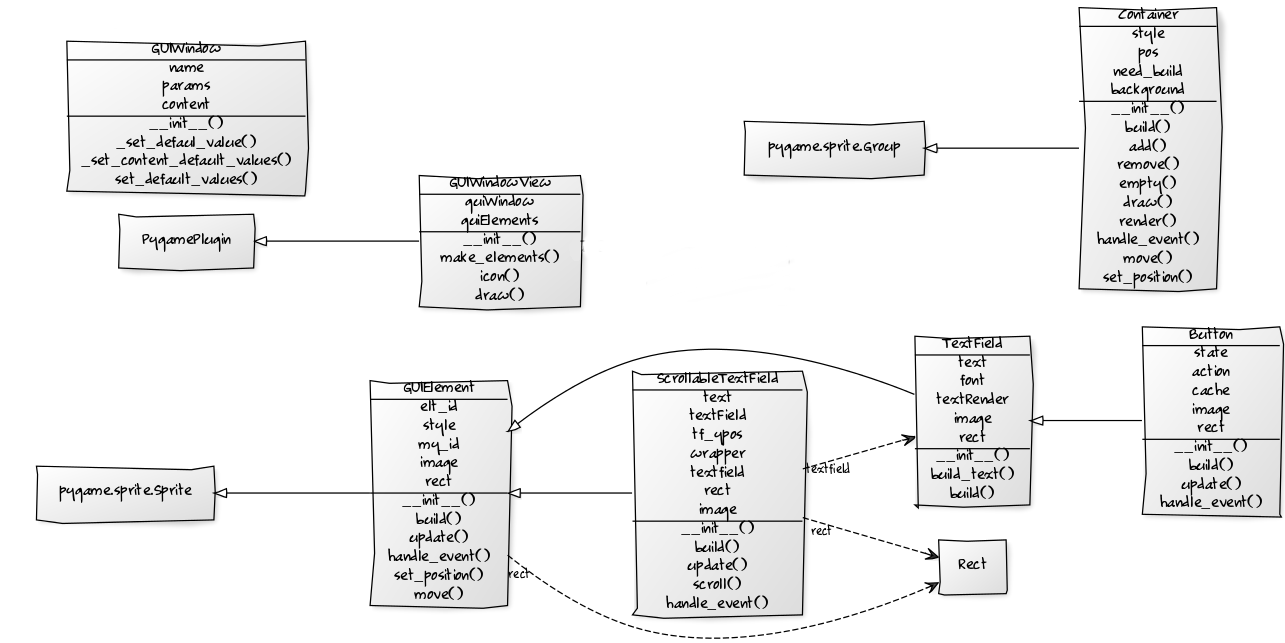
\includegraphics[scale=0.25]{gui_uml.png}\end{center}
\end{frame}

%%%%%%%%%%%%%%%%%%%%%%%%%%%%%%%%%%%%%%%%%%%%%%%%%%%%%%%%%%





\setbeamertemplate{navigation symbols}{} 
\renewcommand{\insertnavigation}[1]{\hfill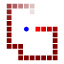
\includegraphics[scale=.5]{main.png}~\vspace{-.2cm}}
\section{Éditeur}

    \begin{frame}
        \frametitle{Contents}
        \tableofcontents[currentsection]
    \end{frame}

\subsection{Objectifs}
\begin{frame}{Objectifs}
	\begin{itemize}
	\item Création des jeux
		\item Modification de jeux (en cours de campagne)
		\item Création de XML pour le serveur et les clients
		\item Utilisation d'abstractions pour l'édition (Ajout de vie, déroulement du temps, ...)
	\end{itemize}
\end{frame}

\subsection{Choix techniques}
\begin{frame}{Outils utilisés}
	\textbf{Langage de programmation :}
	C++
	\begin{itemize}
		\item Sécurité et confort du typage
		\item Performances
		\item Lisibilité du code (.h)
	\end{itemize}
	
	~
	
	\textbf{Interface graphique :}
	Framework Qt
	\begin{itemize}
		\item Connaissances préalables
		\item Outils de création de fenêtre puissant (Qt Designer)
		\item API haut niveau (lecture/écriture XML)
	\end{itemize}
	
	~
	
	\textbf{Inconvénients :} Duplication de code
\end{frame}

\subsection{Architecture}
\begin{frame}{Architecture}
	\textbf{Architecture globale :}
	\begin{itemize}
		\item Modèle :
		\begin{itemize}
			\item Représentation interne des données
			\item Accesseurs et mutateurs pour assurer des invariants
		\end{itemize}
		\item Interface :
		\begin{itemize}
			\item Accès aux données
			\item Ajout et modification d'éléments
			\item Abstractions des mécanismes d'événements et d'actions
		\end{itemize}
	\end{itemize}

\end{frame}

\begin{frame}{Interface}
	\textbf{Architecture Qt classique}
	\begin{itemize}
		\item Sous classe pour les \textit{widgets} d'affichage spécifiques
		\item Utilisation de l'API Model/View
	\end{itemize}
	
	~
	
	\textbf{Patrons de conception utilisés}
	\begin{itemize}
		\item \textit{Fabrique} : Éditeurs spécifiques aux objets
		\item \textit{Singleton} : Options de l'éditeur (dossiers par défaut, ...)
	\end{itemize}
\end{frame}


\begin{frame}{Modèle}
	\textbf{Classe de base : } \texttt{GameObject} 
	\begin{itemize}
		\item Utilisation du polymorphisme (écriture de XML, édition)
		\item Organisation des jeux en arbre
		\item Éléments communs : 
		\begin{itemize}
			\item Paramètres
			\item Drapeaux
			\item Événements
			\item Ordres
		\end{itemize}
		\item Mécanismes d'information des modifications
		\item Facilité de libération de mémoire
		\item Identifiant unique
	\end{itemize}
\end{frame}

\begin{frame}{Modèle}
	\textbf{Héritage d'objet}
	\begin{itemize}
		\item Classe \texttt{InheritableObject}
		\item Distinction \texttt{Type/TypedObject}
		\item Redéfinition des valeurs des paramètres/drapeaux
	\end{itemize}
	
	~
	
	\textbf{Objets virtuels d'organisation :}
	\begin{itemize}
		\item \texttt{DefaultTypes}
		\item \texttt{GameObjectList}
		\item \texttt{GameObjectInventory}
	\end{itemize}
\end{frame}


\begin{frame}{Modèle}
	\textbf{Diagramme des classes}
	
	~
	
	\begin{center}
		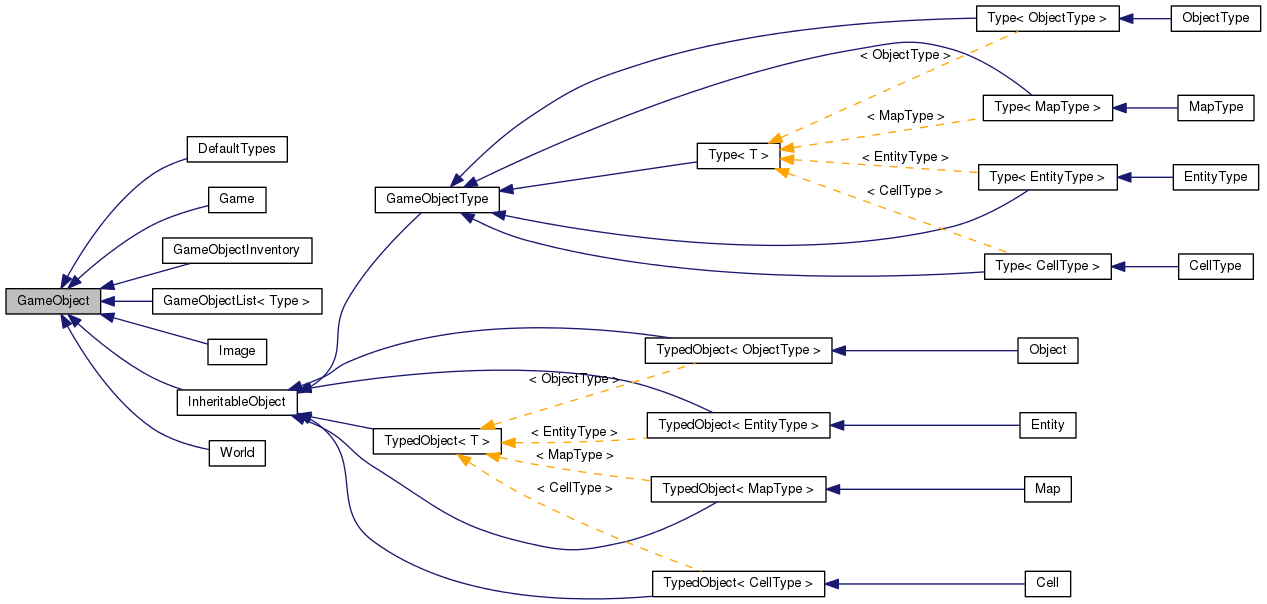
\includegraphics[scale=.24]{GameObject.png}
	\end{center}
\end{frame}


\begin{frame}{XML}
	\textbf{Export}
	\begin{itemize}
		\item XML du serveur : lisible par les serveur/clients
		\item XML de l'éditeur : contient des informations d'édition et d'organisation interne
	\end{itemize}
	
	~
	
	\textbf{Import}
	
	Import de jeux par lecture de XML (éditeur)
\end{frame}


\section{Commentaires}

    \begin{frame}
        \frametitle{Contents}
        \tableofcontents[currentsection]
    \end{frame}
    
\begin{frame}{Difficultés - Choix discutables \textit{a posteriori}}
	\textbf{Pygame}
	\begin{itemize}
		\item efficace pour de petits projets
		\item pas adapté aux moyens/gros projets
		\item quelques problèmes de compatibilité
		\item manque de documentation avancée et/ou d'exemples d'utilisation avancés suffisamment commentés
	\end{itemize}
\end{frame}


\begin{frame}{Remarques}
	\textbf{Général}
	\begin{itemize}
		\item Préciser les architectures avant de coder
		\item Faire avancer les différents composants à la même vitesse
		\item On a sous-estimé la charge de travail liée à l'affichage
		\item[]
		\item Quelques problèmes de communication en cours de route
		\item Gros problème de partage des taches malgré quelques tentatives pour mieux les répartir
		\item[]
		\item difficile à tester
	\end{itemize}
\end{frame}


\begin{frame}{Perspectives}
	\textbf{Interface}
	\begin{itemize}
		\item architecture de l'interface cohérente et pratique
		\item système de plugin tout puissant (tout est modifiable à travers des plugins)
		\item interface soutenable a moyen terme pour des jeux de taille moyenne
	\end{itemize}
	
	~
	
	\textbf{Éditeur}
	\begin{itemize}
		\item Définition d'un langage d'ordre
		\item Ajout d'abstractions dans l'éditeur
		\item Révisions du XML (pour que XML serveur $\subset$ XML éditeur)
	\end{itemize}
\end{frame}


\end{document}
